\documentclass[10pt,a4paper]{report}

\usepackage[utf8]{inputenc}
\usepackage{amsmath}
\usepackage{graphicx}
\usepackage[amsmath,thmmarks]{ntheorem}
\usepackage[all,cmtip]{xy}
\usepackage{cite}
\usepackage{color}
\usepackage{subcaption}
\usepackage[export]{adjustbox}
\usepackage{multirow}
\usepackage[table]{xcolor}

\makeatletter 
 \newtheoremstyle{myu}
  {\item[\hskip\labelsep \ \bf\underline{##1 \theorem@headerfont ##2.}]}
\makeatother
\makeatletter 
 \newtheoremstyle{myn}
  {\item[\hskip\labelsep \ \bf ##1 \theorem@headerfont ##2.]}
\makeatother


\theoremstyle{myn}
\newtheorem{theoremn}{Theorem} 
\theoremstyle{myu}
\newtheorem{theoremu}[theoremn]{Theorem}

\title{LaTeX Document}
\author{Nikita Tyuplyaev}
\date{July 2022}

\begin{document}
\maketitle

\begin{abstract}
\textsf{This is the LaTeX document written by DSBA student Nikita Tyuplyaev, July 2022. This document consists of several parts with scientific (Maths/Informatics/Computer Science) content (theorems/formulas/notations/lemmas) taken from some articles, textbooks, lecture notes and reports. 
\\\texttt{,,Non scholae sed vitae discimus``} }
\end{abstract}

\tableofcontents 

\chapter{The only one chapter}


\section{Linear algebra}

$$\begin{pmatrix}
            5  & -11 & 3 \\
            -13 &   9 & 29 \\
            54  &   0 & 121
        \end{pmatrix}
        \begin{pmatrix}
            x\\ y\\ z
        \end{pmatrix}
        =
        \begin{pmatrix}
           5x-11y+3z \\
           -13x+9y+29z \\
           54x+121z
        \end{pmatrix}$$

\begin{theoremu}
Let $V$, $W$ be two vector spaces. A function $T \colon V \to W$ is called a {\em linear transformation} from $V$ to $W$ if the following hold for all vectors $u, v$ in $V$ and for all scalars $k$.
\begin{itemize}
\item[(i)] $T (u + v) = T (u) + T (v)$
(additivity)

\item[(ii)] $T (k u) = k T (u)$
(homogeneity)
\end{itemize}
\end{theoremu}

\begin{theoremu}
 A function $T \colon V \to W$  is a linear transformation if and only if for all vectors $v_1, v_2$ in $V$ and for all scalars $k_1, k_2$ we have
$$T (k_1 \, v_1 + k_2 \, v_2) = k_1 \, T (v_1) + k_2 \, T (v_2)$$
\end{theoremu}

$$\left( \begin{array}{cccc|c}
             3 & -2 &  1 & -1 &  7\\
            -1 &  0 & -5 &  2 &  2\\
             0 &  1 &  2 &  0 &  0\\ 
            -2 &  3 &  0 & -5 & -1
          \end{array} \right)$$

\begin{theoremu}
    $ V(WHQIC) = 4(\sum \limits _{i=1}^{n}w_{i} ^{2} V(-\log f(x_{i}/\widehat{\theta })) - 2\sum \limits _{i=1}^{n}\sum \limits _{j=1}^{n}E( ((-\log f(x_{i} /\widehat{\theta }) -- E(-\log f(x_{i} /\widehat{\theta })) ((-\log f(x_{j} /\widehat{\theta })-E(-\log f(x_{j} /\widehat{\theta })))) $
\end{theoremu}

$ A_{m,n} = 
 \begin{pmatrix}
  a_{1,1} & a_{1,2} & \cdots & a_{1,n} \\
  a_{2,1} & a_{2,2} & \cdots & a_{2,n} \\
  \vdots  & \vdots  & \ddots & \vdots  \\
  a_{m,1} & a_{m,2} & \cdots & a_{m,n} 
 \end{pmatrix} $

 \clearpage


\section{Calculus}

\begin{theoremn}
\[\int_{x^2 + y^2 \leq R^2} f(x,y)\,dx\,dy
   = \int_{\theta=0}^{2\pi} \int_{r=0}^R
      f(r\cos\theta,r\sin\theta) r\,dr\,d\theta.\]
     \[\int_0^R \frac{2x\,dx}{1+x^2} = \log(1+R^2).\]
      
\end{theoremn}
 
\begin{theoremn}
    
    In non-relativistic wave mechanics, the wave function
$\psi(\mathbf{r},t)$ of a particle satisfies the
\emph{Schr\"{o}dinger Wave Equation}
\[ i\hbar\frac{\partial \psi}{\partial t}
  = \frac{-\hbar^2}{2m} \left(
    \frac{\partial^2}{\partial x^2}
    + \frac{\partial^2}{\partial y^2}
    + \frac{\partial^2}{\partial z^2}
  \right) \psi + V \psi.\] 
It is customary to normalize the wave equation by
demanding that
\[ \int \!\!\! \int \!\!\! \int_{\textbf{R}^3}
      \left| \psi(\mathbf{r},0) \right|^2\,dx\,dy\,dz = 1.\] 
A simple calculation using the Schr\"{o}dinger wave
equation shows that
\[ \frac{d}{dt} \int \!\!\! \int \!\!\! \int_{\textbf{R}^3}
      \left| \psi(\mathbf{r},t) \right|^2\,dx\,dy\,dz = 0,\] 
and hence
\[ \int \!\!\! \int \!\!\! \int_{\textbf{R}^3}
      \left| \psi(\mathbf{r},t) \right|^2\,dx\,dy\,dz = 1\] 
for all times~$t$. If we normalize the wave function in this
way then, for any (measurable) subset~$V$ of $\textbf{R}^3$
and time~$t$,
\[ \int \!\!\! \int \!\!\! \int_V
      \left| \psi(\mathbf{r},t) \right|^2\,dx\,dy\,dz\] 
represents the probability that the particle is to be found
within the region~$V$ at time~$t$.
\end{theoremn}

\[ \lim_{x \to +\infty} \frac{3x^2 +7x^3}{x^2 +5x^4} = 3.\] 

$$\sum_{i=1}^n i^2 = \frac{n(n+1)(2n+1)}{6}$$

\clearpage


\section{Computer Science}

\xymatrix{
U \ar@/_/[ddr]_y \ar@/^/[drr]^x
\ar@{.>}[dr]|-{(x,y)} \\
& X \times_Z Y \ar[d]^q \ar[r]_p
& X \ar[d]_f \\
& Y \ar[r]^g & Z }

\center\textbf{Activity 1.1}

\begin{align*}
&\text{set A is}\ \textit{good} \iff A\  \notin  A.\\
&G\  = \left\{A\bigm|A \ is \ good\right\}\\
&G\  \in \ G?
\end{align*}

\center\textbf{Activity 1.2}

Use the definition of the derivative to find $f'(x)$ when $f(x)=x^{\frac{1}{4}}$.

Using the definition of the derivative, we have
\begin{align*}
            f'(x)           &= \lim_{h\rightarrow 0}\frac{(x+h)^{1/4}-x^{1/4}}{h}   \\
                            &=  \lim_{h\rightarrow 0}\frac{(x+h)^{1/4}-x^{1/4}}{h}\cdot \frac{((x+h)^{1/4}+x^{1/4})((x+h)^{1/2}+x^{1/2})}{((x+h)^{1/4}+x^{1/4})((x+h)^{1/2}+x^{1/2})}\\
                            &=  \lim_{h\rightarrow 0}\frac{(x+h)-x}{h((x+h)^{1/4}+x^{1/4})((x+h)^{1/2}+x^{1/2})}    \\  
                            &=  \lim_{h\rightarrow 0}\frac{1}{((x+h)^{1/4}+x^{1/4})((x+h)^{1/2}+x^{1/2})}   \\
                            &= \frac{1}{(x^{1/4}+x^{1/4})(x^{1/2}+x^{1/2})} \\
                            &=  \frac{1}{(2x^{1/4})(2x^{1/2})}  \\
                            &=  \frac{1}{4x^{3/4}}  \\
                            &=  \frac{1}{4}x^{-3/4}
\end{align*}
Note: the key observation here is that
\begin{align*}
    a^4-b^4 &= (a^2-b^2)(a^2+b^2)   \\
        &= (a-b)(a+b)(a^2+b^2), 
\end{align*}
with 
\[
    a = (x+h)^{1/4}, \qquad b = x^{1/4},
\]
which allowed us to rationalize the denominator.

\clearpage


\section{Support Vector Machine}

\textit{Support Vector Machine or SVM is a supervised and linear Machine Learning algorithm most commonly used for solving classification problems and is also referred to as Support Vector Classification.\cite{noble2006support} There is also a subset of SVM called SVR which stands for Support Vector Regression which uses the same principles to solve regression problems. SVM also supports the kernel method also called the kernel SVM which allows us to tackle non-linearity. The objective of SVM is to draw a line that best separates the two classes of data points.\footnote{SVM finds the hyperplane that best separates the categories in the sense that it maximizes the distance to points in either category} SVM generates a line that can cleanly separate the two classes. How clean, you may ask. There are many possible ways of drawing a line that separates the two classes, however, in SVM, it is determined by the margins and the support vectors. The margin is the area separating the two dotted green lines as shown in the image above. The more the margin the better the classes are separated. The support vectors are the data points through which each of the green lines passes through. These points are called support vectors as they contribute to the margins and hence the classifier itself. These support vectors are simply the data points lying closest to the border of either of the classes which has a probability of being in either one. The SVM then generates a hyperplane which has the maximum margin, in this case the black bold line that separates the two classes which is at an optimum distance between both the classes. In case of more than 2 features and multiple dimensions, the line is replaced by a hyperplane that separates multidimensional spaces. When data are unlabelled, supervised learning is not possible, and an unsupervised learning approach is required, which attempts to find natural clustering of the data to groups, and then map new data to these formed groups. The support-vector clustering[2] algorithm, created by Hava Siegelmann and Vladimir Vapnik, applies the statistics of support vectors, developed in the support vector machines algorithm, to categorize unlabeled data. For instance, an SVM can learn to recognize fraudulent credit card activity by examining hundreds or thousands of fraudulent and nonfraudulent credit card activity reports. Alternatively, an SVM can learn to recognize handwritten digits by examining a large collection of scanned images of handwritten zeroes, ones and so forth. SVMs have also been successfully applied to an increasingly wide variety of biological applications.\cite{noble2004support} A common biomedical application of support vector machines is the automatic classification of microarray gene expression profiles. Theoretically, an SVM can examine the gene expression profile derived from a tumor sample or from peripheral fluid and arrive at a diagnosis or prognosis. Throughout this primer, I will use as a motivating example a seminal study of acute leukemia expression profiles. Other biological applications of SVMs involve classifying objects as diverse as protein and DNA sequences, microarray expression profiles and mass spectra3.\cite{guyon2002gene}
}

\clearpage


\section{SVM images}

\begin{center}
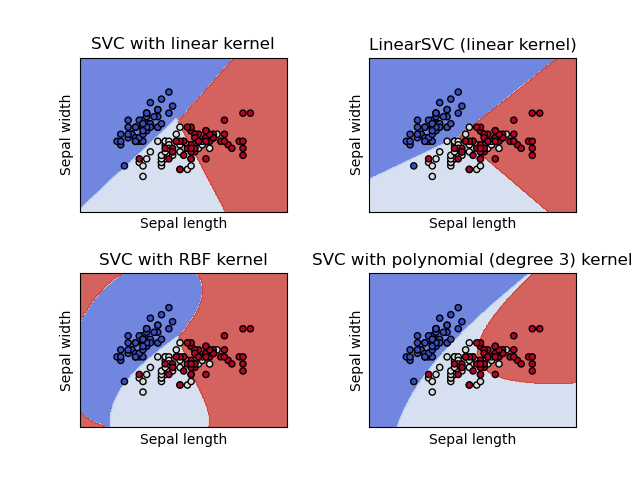
\includegraphics[width=0.9\linewidth, right]{img/img1.png}
\end{center}

\begin{center}
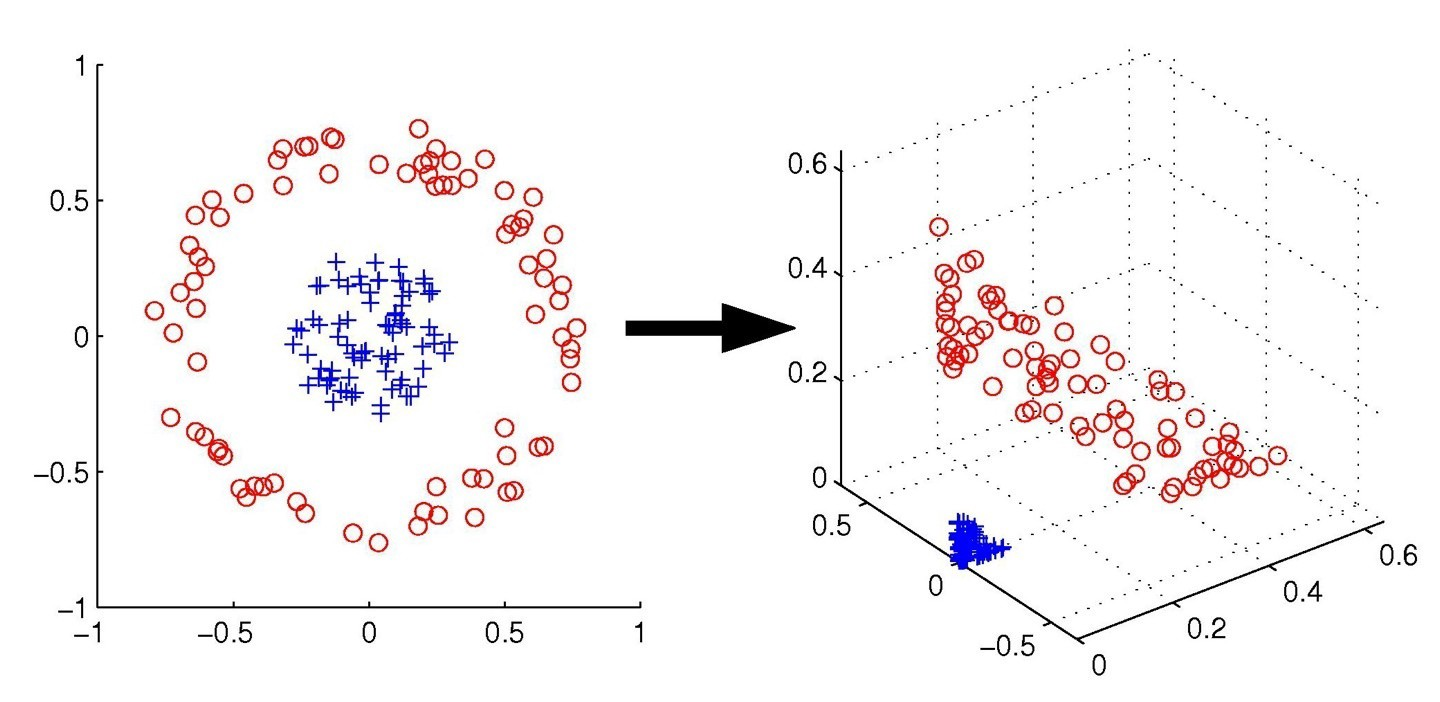
\includegraphics[width=0.9\linewidth, right]{img/img2.jpeg}
\end{center}

\begin{tabular}{c | c c c}
    Original photo & Y-spectrum & U-spectrum & V-spectrum \\ \hline
    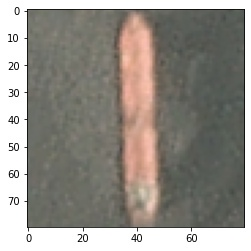
\includegraphics[width=0.25\textwidth, height=30mm]{img/yuv1.jpg} & 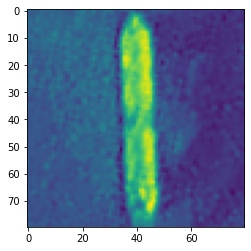
\includegraphics[width=0.25\textwidth, height=30mm]{img/yuv2.jpg} & 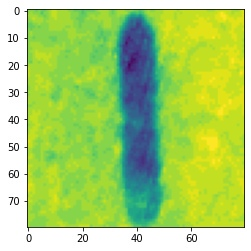
\includegraphics[width=0.25\textwidth, height=30mm]{img/yuv3.jpg} & 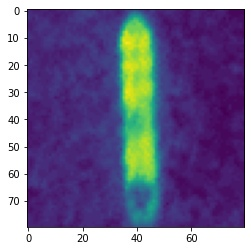
\includegraphics[width=0.25\textwidth, height=30mm]{img/yuv4.jpg} \\
\end{tabular}

\clearpage


\section{Tables and lists}

\begin{center}
\rowcolors{1}{pink}{violet}
\begin{tabular}{||c c c c||} 
 \hline
 Col1 & Col2 & Col2 & Col3 \\ [0.5ex] 
 \hline\hline
 1 & 2 & 3 & 4 \\ 
 \hline
 221 & 7 & 78 & 54 \\
 \hline
 3 & 545 & 778 & 7507 \\
 \hline
 4 & 52 & 1244 & 7587 \\
 \hline
 5786 & 898 & 7878 & 6644 \\ [1ex] 
 \hline
\end{tabular}
\end{center}

\begin{tabular}{ |p{3cm}||p{3cm}|p{3cm}|p{3cm}|  }
 \hline
 \multicolumn{4}{|c|}{Country List} \\
 \hline
 Country Name or Area Name& ISO ALPHA 2 Code &ISO ALPHA 3 Code&ISO numeric Code\\
 \hline
 Afghanistan   & AF    &AFG&   004\\
 Aland Islands&   AX  & ALA   &248\\
 Albania &AL & ALB&  008\\
 Algeria    &DZ & DZA&  012\\
 American Samoa&   AS  & ASM&016\\
 Andorra& AD  & AND   &020\\
 Angola& AO  & AGO&024\\
 \hline
\end{tabular}

\begin{center}
\textsf{Ordered List}
\begin{enumerate}  
\item first point  
\item second point  
\item third point
\end{enumerate} 
\end{center}

\begin{center}
\textsf{Unordered List}
\begin{itemize}  
\item first point  
\item second point  
\item third point
\end{itemize} 
\end{center}

\begin{center}
\textsf{Nested List}
\begin{enumerate}
   \item first item
   \item first item
   \begin{enumerate}
     \item second item
     \item second item
     \begin{enumerate}
       \item third item
       \item third item
       \begin{enumerate}
         \item fourth item
         \item fourth item
       \end{enumerate}
     \end{enumerate}
   \end{enumerate}
 \end{enumerate}
\end{center}
 
\bibliographystyle{plain}
\bibliography{main.bib}

\end{document}
